\paragraph{Parallel axis}
For constant $\omega$, for two parallel axis $I$ and $I_c$, which goes throw center of the body, with distance $l$ between them for body of total mass $M$ moment of inertia is
$$I_c = \sum_i m_i r_{icm}^2$$
$$I = I_c + Mr^2$$

And kinetic energy is:

$$K = \underbrace{K_c}_{\parbox{2cm}{\scriptsize \centering kinetic energy as a result of movement relative to center of mass}} + \underbrace{\frac{1}{2}mv_{cm}^2}_{\parbox{2cm}{\scriptsize \centering kinetic energy as a result of movement of body}}$$

So angular momentum is:

$$\vec{J} = I\vec{\omega} = I_c\vec{\omega}+ Ml^2\vec{\omega}$$

And more general expression for kinetic energy:
$$K = \frac{1}{2}I\vec{\omega} = \underbrace{\frac{1}{2}I_c \omega^2}_{\parbox{2cm}{\scriptsize \centering kinetic energy as a result of movement relative to center of mass}} + \underbrace{\frac{1}{2}Ml^2\omega^2}_{\frac{1}{2}mv_{cm}^2}$$

\subparagraph{Kinetic energy}

$$K = \frac{1}{2} \sum m_i v_i^2 = \frac{1}{2} \sum_i m_i \left( \underbrace{\vec{v}_{icm}}_{\parbox{2cm}{\scriptsize \centering velocity of point i relative to cm}} + \underbrace{\vec{v}_{cm}}_{\parbox{2cm}{\scriptsize \centering velocity of cm}} \right)^2$$

$$K = \frac{1}{2} \sum_i m_i \left( \vec{v}_{icm} + \vec{v}_{cm}\right)\cdot \left( \vec{v}_{icm} + \vec{v}_{cm}\right) = \underbrace{\frac{1}{2}\sum_i m_i v_{icm}^2}_{\parbox{2cm}{\scriptsize \centering kinetic energy as a result of movement relative to center of mass}} + \frac{1}{2}\sum_i m_i v_{cm}^2 + \sum_i \underbrace{m_i \vec{v}_{icm}}_{\parbox{2cm}{\scriptsize \centering 0 since $\vec{p}$ relative to cm is 0}}\vec{v}_{cm} $$

\paragraph{Perpendicular axis}
Two axis in plane of body perpendicular to each other. Moment of inertia relative to them is $I_1$ and $I_2$, while $I_z$ is moment of inertia relative to third axis perpendicular to the plane of the body.

Since $x^2+y^2 = r^2$:
$I_z  = I_1+I_2$.
\paragraph{Examples of values of $I$}
\subparagraph{Examples for the ring}
\begin{enumerate}
	\item Axis perpendicular to plane of ring passing through center of the ring:
	
	$$I_c = MR^2$$
	\item Axis in plane of ring passing through center of the ring:
	
	$$I_1 = \frac{1}{2}MR^2$$
	\item Axis perpendicular to plane of ring passing through surface of the ring:
	
	$$I = I_c + Ml^2 = 2MR^2$$
\end{enumerate}
\subparagraph{Examples for the hard rod}

\begin{center}
	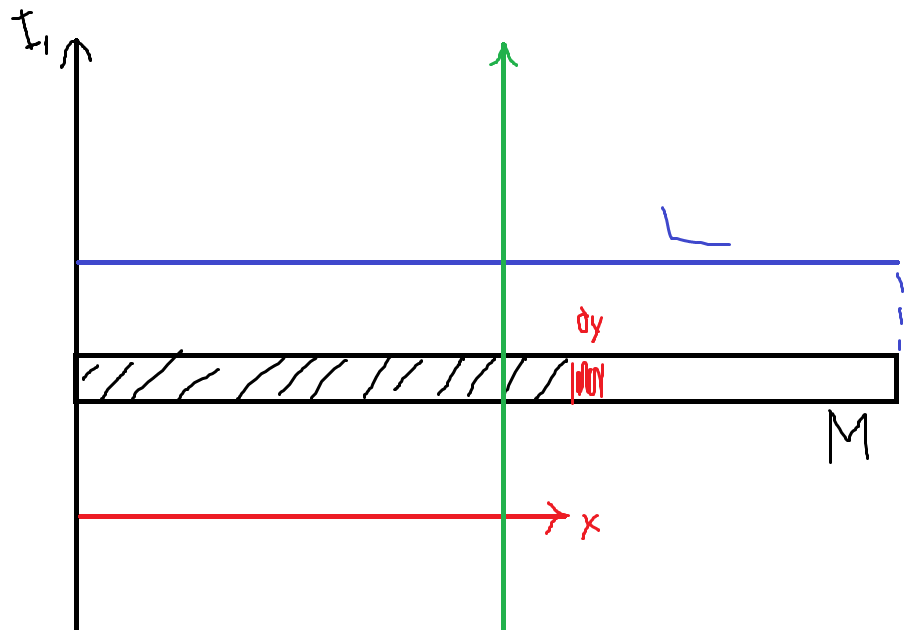
\includegraphics[width=0.9\linewidth]{./lect17/pic1.png}
\end{center}

\begin{enumerate}
	\item Axis in the end of the rod ($I_1$):
	$$I = \sum_i m_i d_i^2$$
	
	For continuous body $\sum \to \int$, $d_i \to x$, $m_i \to \frac{M}{L}dx$:
	
	$$I = \int_{x=0}^{x=L} x^2 dm  = \int_{x=0}^{x=L} x^2 \frac{M}{L}dx= \frac{1}{3}ML^2 $$
	
	\item Axis in the middle of the rod ($I_2$):

	$$\frac{1}{12}ML^2 $$
\end{enumerate}

\subparagraph{Examples for the disc}

\begin{enumerate}
	\item Axis perpendicular to plane of disc passing through center of the ring:
	
	$$I_c = \frac{1}{2}MR^2$$
	\item Axis in plane of disc passing through center of the ring:
	
	$$I_1 = \frac{1}{4}MR^2$$
\end{enumerate}

\subparagraph{Examples for the rectangular plate}
Of size $a\times b$.
\begin{enumerate}
	\item Axis in plane of plate passing through center of the ring:
	$$I_x = \frac{1}{12}Ma^2$$
	$$I_y = \frac{1}{12}Mb^2$$
	
	\item Axis perpendicular to plane of ring passing through center of the ring:
	$$I_z = I_x + I_y$$
\end{enumerate}


\subparagraph{Examples for the sphere}
With constant density $\rho = \frac{M}{\frac{4\pi}{3}R^3}$.
\begin{enumerate}
	\item Axis passing through center of the sphere:
	$$I_z = \frac{2}{5}MR^2$$
\end{enumerate}

\paragraph{Problems with constant axis of rotation}
Equation of the movement is:

$$\frac{d\vec{J}}{dt}= \vec{N} = \vec{r} \times \vec{F}$$

which is equivalent to second law.

\begin{center}
	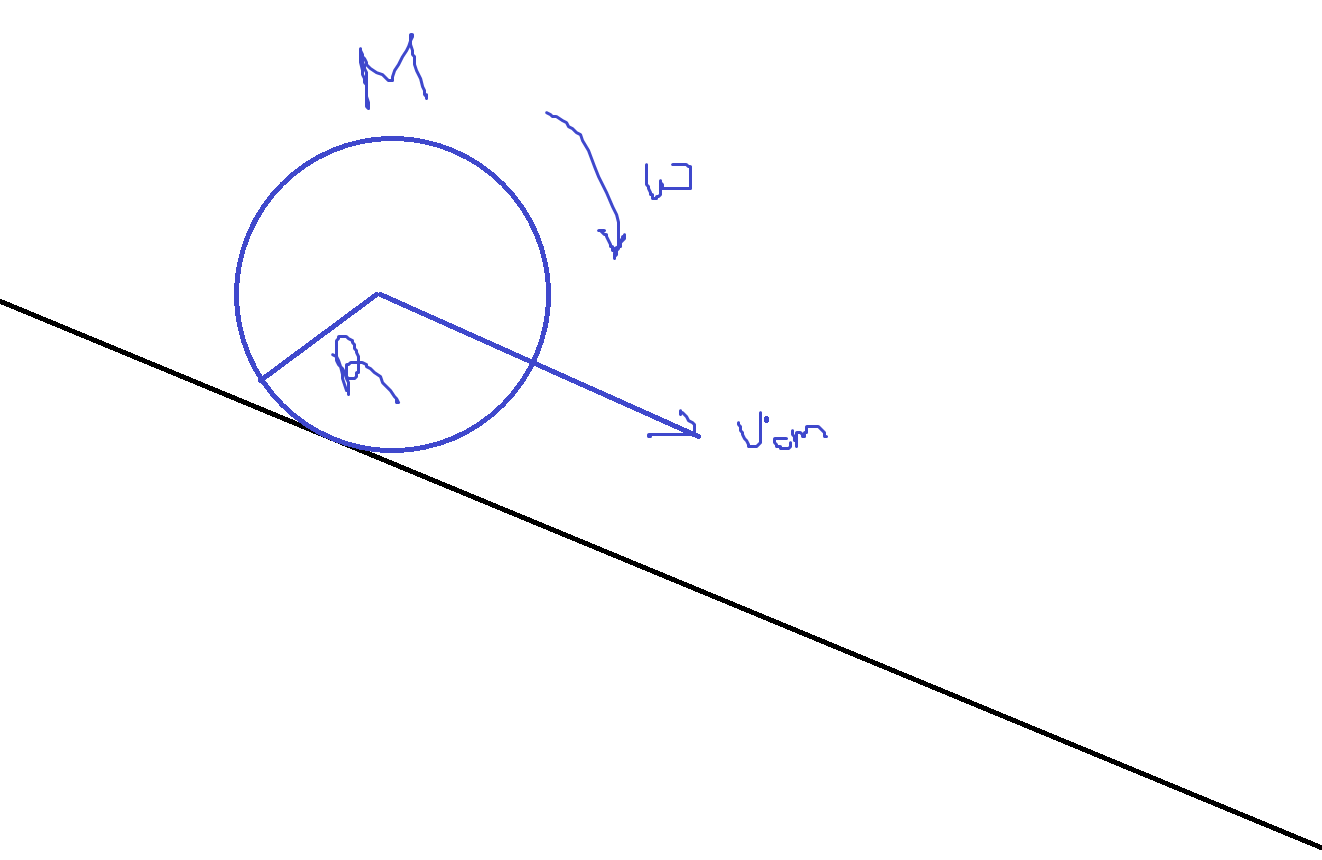
\includegraphics[width=0.9\linewidth]{./lect17/pic2.png}
\end{center}

Kinetic energy of rolling body is:

\begin{align*}
K = K_c + \frac{1}{2}mv^2_{cm} = \frac{1}{2} I_c \omega^2 + \frac{1}{2} m R^2 \omega^2 =\\= \frac{1}{2}I_c \left( \frac{v_cm}{R} \right) \frac{1}{2}mv_{cm}^2 = \frac{1}{2}\left( \frac{I_c}{R^2} + M \right)v_{cm}^2
\end{align*}
